%% La letra n con tilde es: 'n.

\chapter{Background}

This chapter present the fundamental concepts related this work. The formal
definitions referring to fuzzy logic, contexts classification and the
recommender system techniques used in the proposed method.

\section{Fuzzy Logic}

\textbf{Fuzzy logic} originates on 1965 from the publication “Fuzzy
Sets”\cite{zadeh1965fuzzy} written by Lofti A. Zadeh from the University of
Berkeley California for the journal Information and Control, based on
the work of J. Lukasiewicz\cite{saffiotti1995multivalued} about
multi-valuated logic. In contrast with traditional logic, that uses
absolute concepts when it refers to the real world, fuzzy logic
defines these concepts with variable degrees of belonging, following
the reasoning patterns of human thought. \\  

A distictive property of computational systems based on fuzzy logic theory 
is that, unlike those based on classical logic, they have the ability to
acceptably reproduce a more natural form of reasoning, that considers the
certainty of a proposition as a matter of degree. More formally we can
say that if the logic is the science of the formal principles and
policy reasoning, fuzzy or fuzzy logic refers to the formal principles
of approximate reasoning, considering precise reasoning (classical
logic) as a restrictive case. Thus, the most convenient features of fuzzy
logic are its flexibility, tolerance for imprecision, its ability to
model nonlinear problems and its roots in natural language. Although
fuzzy logic is known by this name since the seminal work of Zadeh in
1965, the idea that lies behind it, and its origins date back to 2500
years ago. The Greek philosophers, including Aristoteles, believed
that there were certain degrees of truthfulness and falsehood and
even Platon worked with membership degrees.\\ %Referencias de esto de Aristo y Platon
\textbf{Fuzzy logic} has acquired a great reputation for the variety
of its applications, which range from the control of complex industrial
processes, device design to controlers of household electronics and
entertainment devices, as well as diagnostic systems.  Fuzzy logic is
essentially a \textbf{multi-valued logic}\cite{zadeh1965fuzzy}, which
is an extension of classical logic. The latter imposes on their
statements only true and false values, however, much of human
reasoning is not as 'deterministic´. The word fuzzy can be defined as:
vague or confusing. 
%Fuzzy Systems
Fuzzy systems are \textbf {knowledge-based systems}
or \textbf{rule-based systems}. The kernel (core) of the fuzzy system
consists of knowledge bases called \textbf {IF-THEN} fuzzy rules.
Each fuzzy system is associated with a set of rules with a variety of %¿Como una variedad de representaciones?
representations, as in Figure \ref{fig:fuzzyset} i, which can be
obtained from numerical data or experts familiar with the problem at
hand. 
%No se entiende muy bien, hay que explicar lo de funcion de membresía 
%Variable linguistica y ya después las reglas. 
% basate en mi articulo de http://citeseerx.ist.psu.edu/viewdoc/download?doi=10.1.1.136.3578&rep=rep1&type=pdf 
% sección 2 
Based on this information, actions are combined with background
formatting rules/consequent, and then are added according to the
theory of approximate reasoning to produce a nonlinear mapping of the
input space $ U=U_1 xU_2 x…U_n$ the output space V, where $
F_k^l⊂U_k,k=1,2,…n,$ membership functions are type-1 antecedent, and $
G^1⊂V $ is the membership function of type-1 consistent. The
linguistic variables\cite{dubois1980fuzzy} are denoted by input $uk,
=1,2,…n $, and output linguistic variables are denoted by: $R^l: if
x_1$ is $F_1^l $ and $x_{2}$ is $F_2^l$ and ... and $x_n$ is $F_n^l$
then V is $G^1$.\\ A fuzzy system consists of four basic elements
shown in Figure \ref{fig:fuzzyset}: fuzzifier type-1, the fuzzy rule
base, inference machine and defuzzifier type-1. The \textbf{fuzzy
rule} is a collection of rules, which are combined in the inference
machine to produce a fuzzy output. The fuzzifier maps numeric entries
to fuzzy sets, which are then used as inputs to the inference engine,
where the defuzzifier maps the fuzzy sets produced by the inference
engine to traditional numbers.
\begin{figure*} \captionsetup{justification=centering,margin=2cm} 
\centering
\setlength\fboxsep{0pt} \setlength\fboxrule{0.7pt}
\fbox{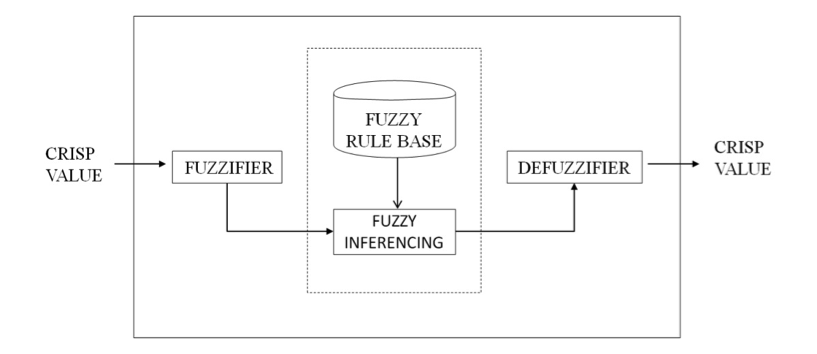
\includegraphics[width=0.75\textwidth]{img/fuzzy1.png}} 
\caption{Estructure of a fuzzy logic system.}
\label{fig:fuzzyset} 
\end{figure*} 

\section{Context}
%%
%% Escribe aquí una intro general de contexto,
%% antes de ver especificamente al contexto en SR 
%% Context y Contextual Information son dos términos distintos
%% Context es el contexto real y de este se extrae información contextual.
%% A veces los usas como si fuera lo mismo. 

%% También debes definir Contextual Factors, creo que es 
%% Información Contextual que puede afectar a la recomendación   

The application of contextual information in recommender systems, there are %
previous approaches by assuming the existence of certain contextual         % Mejorar
factors, such as time, location, and the purchasing purpose, that
identify the context in which recommendations are provided. An
assumption for each of these contextual factors can have a structure;
the time factor, for instance, it can be defined in terms of seconds,
minutes, hours, days, months, and years. The classification of context 
%Segura que es la clasificacion de context?
%Este parrafo es incorrecto
%La enumeración no es una clasificación 
that is proposed by Adomavicious\cite{adomavicius2011context} is based on the 
following two aspects of contextual factors: 1) what a RS may know
about these contextual factors and, 2) how contextual factors change
over time.
\begin{enumerate}

%% Este parrafo repite habla de la clasificación, no es una clasificación
\item \textbf{What a recommender system may know about these contextual factors.} 
A recommender system can have different types of knowledge, which may include 
the exact list of all the relevant factors, their structure, and their values, 
about the contextual factors. Depending on what exactly the system knows (that 
is, what is being observed), it can classify the knowledge of a recommender 
system about the contextual factors into three categories: 
	%% Entonces se clasifican en tres:
	\begin{itemize}
	\item \textbf{Fully observable}: The contextual factors relevant to the 
	application, as well as their structure and their values at the time when 
	recommendations are made, are known explicitly. For example, when
	recommending the purchase of a certain product, like a shirt, the 
	recommender system may know only the \tt{Time}, PurchasingPurpose, and  %% Ponlos como \tt{}
	ShoppingCompanion factors matter in this application. Further, the 
	recommender system may know the structure of all these three contextual 
	factors, such as having categories of weekday, weekend, and holiday for 
	Time. Further, the recommender system may also know the values of the 
	contextual factors at the recommendation time (for example, when this 
	purchase is made, with whom, and for whom).
	\item \textbf{Partially observable}: Only some of the information about 
	the contextual factors described above, is explicitly known. For example, 
	the recommender system may know all the contextual factors, such as Time, 
	PurchasingPurpose, and ShoppingCompanion, but not their structure. Note that 
	there can possibly be different levels of “partial observability.” In this 
	article we do not differentiate between them and group various cases of 
	partially observable knowledge into this general category.
	\item \textbf{Unobservable}: No information about contextual factors is 
	explicitly available to the recommender system, and it makes recommendations 
	by utilizing only the latent knowledge of context in an implicit manner. 
	For example, the recommender system may build a latent predictive model, 
	such as hierarchical linear or hidden Markov models, to estimate unknown 
	ratings, where unobservable context is modeled using latent variables.
	\end{itemize}
\item \textbf{How contextual factors change over time.} Depending on whether 
contextual factors change over time or not, there are two categories: 
	\begin{itemize}
	\item \textbf{Static}: The relevant contextual factors and their structure
	remains the same (stable) over time. For example, in case of recommending a
	purchase of a certain product, such as a shirt, we can include the
	contextual factors of Time, PurchasingPurpose, ShoppingCompanion and only
	them during the entire lifespan of the purchasing recommendation
	application.
	\item \textbf {Dynamic}: This is the case when the contextual factors change in 
	some way. For example, the recommender system (or the system designer) may 
	realize over time that the ShoppingCompanion factor is no longer relevant for 
	purchasing recommendations and may decide to drop it. Furthermore, the structure 
	of some of the contextual factors can change over time (for example, new 
	categories can be added to the PurchasingPurpose contextual factor over time).
	\end{itemize}
\end{enumerate} 
On the other hand, Fling\cite{fling2009mobile} considers four types of context that 
can be used by different applications:  %Creo que estos pueden ser factores, no contextos 
\begin{itemize} 
\item \textbf{Physical context}: representing the time, position, and activity 
of the user, but also the weather, light, and temperature when the 
recommendation is supposed to be used. 
\item \textbf{Social context}: representing the presence
and role of other people (either using or not using the application) around the
user and whether the user is alone or in a group when using the application.
\item \textbf{Interaction media context}: describing the device used to access
the system (for example, a mobile phone or a kiosk) as well as the type of media
that are browsed and personalized. The latter can be ordinary text, music,
images, movies, or queries made to the recommender system. 
\item \textbf{Modal context}: representing the current state of mind of the user, 
the user’s goals, mood, experience, and cognitive capabilities.  
\end{itemize}
The contexts classification reachs to a general context definition %No se si llamarle clasificacion
adopted like the most suitable definition proposed by A. K. Dey  and it
was mentioned in chapter 1.\\ 

%% Esta idea es tuya? Creo que yo no llamaría a esto context más bien algo como context factor  
Then, an example to explain context is considering a context-aware
application, an indoor mobile tour guide. Here, the
entities are the user, the application and the tour sites.  We will
look at two pieces of information – weather and the presence of other
people – and use the definition to determine if either one is context.
The weather does not affect the application because it is being used
indoors. Therefore, it is not context. The presence of other people,
however, can be used to characterize the user’s situation. If a user
is traveling with other people, then the sites that they visit may are
the points of interest for the user. Therefore, the presence of other
people is context because it can be used to characterize the user’s
situation. \\ 
%Falta afinar el siguiente párrafo:
Previously understanding the context, it is likely to define \textbf
{context-aware recommender systems}, it is viable to adopt the
definition of \textbf{A. K. Dey et.al}\cite{dey2001understanding} to
formalize what features it has a Context-aware recommender
system:\textit{``a system is context-aware if it uses context to
provide relevant information and/or services  to the user, where
relevancy depends on the user’s task."} \\  This definition is closer
to the real about behaviour of \textbf{context-aware recommender
system} when it incorporates contextual information to get
recommendations,  in addition, is fewer confused and specific than
other author's definitions.

\section{Recommender systems}

\subsection{Collaborative Filtering algorithm}

The idea of collaborative recommendation approaches is to exploit
information about the past behavior or the opinions of an existing
user community for predicting which items the current user of the
system will most probably like or be interested in
\cite{anIntroduction}. Recommender systems are useful in several types
of  applications, however, the big impact is mainly in web sites for
sales in order to  personalize the information for a particular user,
then the system helps to  promote another items to grow up the sales
in the on-line storage. Collaborative filtering  take a matrix of
given \textit{user-item} ratings as the input to generate a prediction
for each item  indicating to what degree the current user will like or
dislike  an item, subsequently the list of \textit{n} recommended %ajustar
items for the user that contains items no reviewed by the user.
Differents approaches are utilized for collaborative filtering such
as:  a) user-based nearest neighbor recommendation, b) Item-based
nearest neighbor  recommendation and c) model-based recommendation.\\
a) \textit{User-based nearest neighbor} is the most used approach because
of is easy of implementation and efficient results. Only need the
rating matrix to obtain recommendations for users. The neighborhood
selection is taking the \textit{K} nearest neighbors into account
usind the threshold to define  the size of the neighborhood. A reduced
size of neigborhood can not make predictions, on the  contrary, is the
neighborhood is large the information for recommendations can not be
significant.\\ To obtain the similarity value between user and
neighbors, the Pearson correlations measure is used, takes values from
$+1$ (strong positive correlation) to $-1$ (strong negative
correlation) to define how similar a neighbor is. The similarity
$sim(a,b)$ of users $a$ and $b$, given the rating matrix $R$ is
denoted by the following equation:
\begin{equation}\label{eq:pearson1}
\displaystyle sim(a,b) = {\sum_{p \in P}(r_{a,p} - 
\bar{r_a})(r_{b,p}- \bar{r_b}) 
\over \sqrt{\sum_{p \in P}(r_{a,p} - \bar{r_a})^2} 
\sqrt{\sum_{p \in P} 
(r_{b,p}- \bar{r_b})^2}}
\end{equation}
Where the symbol $\bar{r_a}$ corresponds to the average rating of user
$a$. Subsequently, a formula to calculate the prediction of the user
$a$ for item $p$ that also factors the relative proximity of the
nearest neighbors $N$ and $a's$ average rating $\bar{r_a}$ is denoted
by the following equation:
\begin{equation}\label{eq:prediction}
\displaystyle pred(a,b) = \bar{r_a} + 
{\sum_{b \in N} sim(a,b) * (r_{b,p}- \bar{r_b}) 
\over \sum_{b \in N} sim(a,b)} 
\end{equation}
b) \textit{Item-based nearest neighbor} is the same idea than the \textit
{user-based}, the difference is that the approach tries to find
similar items in place of similar users to get information of rating
matrix.  Then, the idea of \textit{item-based} is to compute
predictions using the similarity between items and not the similarity
between users.  To find similar items cosine similarity measure is
defined, this metric measures the similarity between two
\textit{n-dimensional} vectors based on the angle between them.
Therefore, the similarity between two items \textit{a} and \textit{b}
– viewed as the corresponding rating vectors $a$ and $b$ – is formally
defined as follows:
\begin{equation}\label{eq:cosine}
\displaystyle sim(\overrightarrow{a},\overrightarrow{b})= 
{\overrightarrow{a}* \overrightarrow{b} \over
|\overrightarrow{a}|*|\overrightarrow{b}| }
\end{equation}
The * symbol is the dot product of vectors. $|a|$ is the Euclidian
length of the vector, which is defined as the square root of the dot
product of the vector with itself.\\ 
c) \textit{Model-based approach}, in this technique  the raw data are
first processed offline, as described for \textit {item-based}
filtering or some dimensionality reduction techniques. At run time,
only the learned model is required to make predictions. Although
\textit{memory-based} approach is theoretically more precise because
full data is available for generating recommendations, such systems
face problems of scalability when databases of tens of millions of
users and items are used. An example of this approach is matrix
factorization or latent factors model, normally used to fill a rating
matrix to calculate predictions taking in account the latent factors.

\subsection{Content-based algorithm}

In content-based the recommendation task then consists of determining the
items that match the user’s preferences best. Although such an approach must
rely on additional information about items and user preferences, it does not
require the existence of a large user community or a rating history –that is,
recommendation lists can be generated even if there is only one single user. In
practical settings, technical descriptions of the features and characteristics
of an item– such as the genre of a book or the list of actors in a movie – are
more often available in electronic form, as they are partially already provided
by the providers or manufacturers of the goods. What remains challenging,
however, is the acquisition of subjective, qualitative features. In domains of
quality and taste, for example, the reasons that someone likes something are not
always related to certain product characteristics and may be based on a
subjective impression of the item’s exterior design.   \\
\textbf{Content representation.} The simplest way to describe catalog items is
to maintain an explicit list of features for each item (also often called
attributes, characteristics, or item profiles). For a book recommender, one
could, for instance, use the genre, the author’s name, the publisher, or
anything else that describes the item and store his information in a relational
database system. When the user’s preferences are described in terms of his or
her interests using exactly this set of features, the recommendation task
consists of matching item characteristics and user preferences.  \\
\textbf{Vector space model.}  Content-based systems have historically been
developed to filter and recommend text-based items such as e-mail messages or
news. The standard approach in CB recommendation is, therefore, not to maintain
a list of \textit{meta-information features}, but to use a list of relevant keywords
that appear within the document. The main idea, of course, is that such a list
can be generated automatically from the document content itself or from a 
free-text description thereof.

\subsection{Hybrid recommender systems} 

Each recommender system technique has its pros and cons – for
instance, the ability to handle data sparsity and cold-start problems
or considerable efforts for knowledge acquisition and engineering. \\ 
User models and contextual information, community and
product data, and knowledge models constitute the potential types of
recommendation input. However, none of the basic approaches is able to
fully exploit all of these. Consequently, building hybrid systems that
combine the strengths of different algorithms and models to overcome
some of the afore mentioned shortcomings and problems has become the
target of recent research. Hybrid recommender systems are technical
approaches that combine several algorithms or recommendation components.

\subsection{Context-aware recommender systems}

Traditionally, the recommendation problem has been viewed as a prediction
problem in which, given a user profile and a target item, the recommender
system’s task is to predict that user’s rating or that item, reflecting the
degree of user’s preference for that item. \\  Specifically, a recommender system
tries to estimate a rating function:  $R$ : $Users * Items$ $ 
\leftarrow Ratings$, that maps \textit{user-item} pairs to an ordered 
set of rating values.\\ 
In contrast to the traditional model, context-aware recommender system tries to
incorporate or utilize additional evidence (beyond information about users and
items) to estimate user preferences on unseen items. \\ When such contextual
evidence can be incorporated as part of the input to the recommender systems,
the rating function can be viewed as  \textit{multidimensional}: $R$ : $Users *
Items * Contexts$ $ \leftarrow Ratings$, where \textbf{contexts} represents a set of
factors that further delineate the conditions under which the \textit{user-item}
pair is assigned a particular rating. \\ The underlying assumption of this extended
model is that user preferences for items are not only a function of items
themselves, but also a function of the context in which items are being
considered\cite{lim2009assessing}.

\subsection{Paradigms}

When recommender system uses the contextual information, it starts
with the data having the form \textit{U * I * C * R}, where \textit{C}
is additional contextual   dimension and end up with a list of
contextual recommendations  $i_{1}$,$i_{2}$,$i_{3}$...$i_{n}$ for each
user. However, when the recommendation process does not take into
account  the contextual information, is posible to apply the
information about the current (or desired) context \textit{c} in
various stages of the recommendation process.  Adomavicious defines
three paradigms to the context-aware recommendation process that is
based on contextual user preference:

\begin{itemize}
\item  \textbf{Contextual pre-filtering (or contextualization of
recommendation input).} In this recommendation paradigm, contextual
information drives data selection or data construction for that specific
context. In other words, information about the current context c is used for
selecting or constructing the relevant set of data records (i.e., ratings).
Then, ratings can be predicted using any traditional 2D recommender system 
on the selected data. 
 	
\item \textbf{Contextual post-filtering (or contextualization of recommendation
output).} In this recommendation paradigm, contextual information is initially
ignored, and the ratings are predicted using any traditional 2D recommender
system on the entire data. Then, the resulting set of recommendations is
adjusted (contextualized) for each user using the contextual information.
\item \textbf{Contextual modeling (or contextualization of recommendation
function).} In this recommendation paradigm, contextual information is used
directly in the modeling technique as part of rating estimation.
\end{itemize}



